\documentclass[11pt]{article}
\usepackage[a4paper,margin=1in]{geometry}
\usepackage{amsmath,amssymb,amsthm}
\usepackage{tikz}
\usepackage{booktabs}
\usepackage{xcolor}
\usepackage[hidelinks]{hyperref}
\hypersetup{pdftitle={Polyomino rectangles by parity},pdfauthor={Vamshi Jandhyala}}
\setlength{\parskip}{0.4em}
\setlength{\parindent}{0pt}

\newtheorem{theorem}{Theorem}
\newtheorem{proposition}{Proposition}
\newtheorem{lemma}{Lemma}

\definecolor{inkblue}{RGB}{40,76,105}
\definecolor{softblue}{RGB}{226,235,243}
\definecolor{rust}{RGB}{153,70,45}

\title{Polyomino rectangles by parity: \\ no rectangle for 8, 10 or 16 cells}
\author{Vamshi Jandhyala}
\date{}

\begin{document}
\maketitle
\vspace{-2em}

\begin{abstract}
For which $n$ can one copy of every hole-free $n$-omino tile a rectangle? On MathOverflow the answer is known to
be yes for $n=1,2,5,7$, no for $n=3,4,6$ and no for $n\ge17$; the cases $8\le n\le16$ were open. We show that the
answer is no for $n=8$, $10$ and $16$. The reason is the checkerboard count that already rules out $4$ and $6$:
with $n$ even, the imbalances of the pieces must add up to a multiple of $4$, and for these three sizes their total is
$2$ modulo $4$. The totals come from two independent enumerations of the $363$, $4460$ and $11\,230\,003$ pieces.
For $n=12$, $14$ and every odd $n$ the count gives no obstruction, so $9$, $11$, $12$, $13$, $14$ and $15$ remain
open. The argument is checked in the Lean proof assistant.
\end{abstract}

\section{The question}

An $n$-omino is a connected set of $n$ unit squares of the grid, and it is hole-free if its complement is
connected. Ralph Morrison asked on MathOverflow~\cite{MO} for which $n$ one copy of each hole-free $n$-omino, up to
rotation and reflection, can tile a rectangle. The answer is yes for $n=1$, $2$, $5$ and $7$, by explicit tilings,
and no for $n=3$, $4$ and $6$. The answers to the question show that it is no for every $n\ge18$ (Budd and Lehner)
and, by a computer count, for $n=17$ (Hoffman). That left $8\le n\le 16$.

Here is the case $n=4$. Colour the grid like a chessboard. Four of the five tetrominoes cover two black and two
white squares wherever they are put; the T-tetromino covers three of one colour and one of the other
(Figure~\ref{fig:pieces}). Stop and decide before reading on: why can the five never fill a rectangle?

\begin{figure}[ht]
\centering
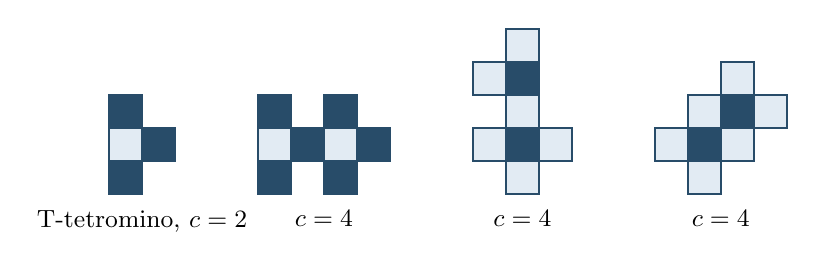
\begin{tikzpicture}[x=0.42cm,y=0.42cm]
  \fill[inkblue,draw=inkblue,thick] (0,0) rectangle ++(1,1);
  \fill[softblue,draw=inkblue,thick] (0,1) rectangle ++(1,1);
  \fill[inkblue,draw=inkblue,thick] (0,2) rectangle ++(1,1);
  \fill[inkblue,draw=inkblue,thick] (1,1) rectangle ++(1,1);
  \node[below,font=\small] at (1.0,-0.2) {T-tetromino, $c=2$};
  \fill[inkblue,draw=inkblue,thick] (4.5,0) rectangle ++(1,1);
  \fill[softblue,draw=inkblue,thick] (4.5,1) rectangle ++(1,1);
  \fill[inkblue,draw=inkblue,thick] (4.5,2) rectangle ++(1,1);
  \fill[inkblue,draw=inkblue,thick] (5.5,1) rectangle ++(1,1);
  \fill[inkblue,draw=inkblue,thick] (6.5,0) rectangle ++(1,1);
  \fill[softblue,draw=inkblue,thick] (6.5,1) rectangle ++(1,1);
  \fill[inkblue,draw=inkblue,thick] (6.5,2) rectangle ++(1,1);
  \fill[inkblue,draw=inkblue,thick] (7.5,1) rectangle ++(1,1);
  \node[below,font=\small] at (6.5,-0.2) {$c=4$};
  \fill[softblue,draw=inkblue,thick] (11.0,1) rectangle ++(1,1);
  \fill[softblue,draw=inkblue,thick] (11.0,3) rectangle ++(1,1);
  \fill[softblue,draw=inkblue,thick] (12.0,0) rectangle ++(1,1);
  \fill[inkblue,draw=inkblue,thick] (12.0,1) rectangle ++(1,1);
  \fill[softblue,draw=inkblue,thick] (12.0,2) rectangle ++(1,1);
  \fill[inkblue,draw=inkblue,thick] (12.0,3) rectangle ++(1,1);
  \fill[softblue,draw=inkblue,thick] (12.0,4) rectangle ++(1,1);
  \fill[softblue,draw=inkblue,thick] (13.0,1) rectangle ++(1,1);
  \node[below,font=\small] at (12.5,-0.2) {$c=4$};
  \fill[softblue,draw=inkblue,thick] (16.5,1) rectangle ++(1,1);
  \fill[softblue,draw=inkblue,thick] (17.5,0) rectangle ++(1,1);
  \fill[inkblue,draw=inkblue,thick] (17.5,1) rectangle ++(1,1);
  \fill[softblue,draw=inkblue,thick] (17.5,2) rectangle ++(1,1);
  \fill[softblue,draw=inkblue,thick] (18.5,1) rectangle ++(1,1);
  \fill[inkblue,draw=inkblue,thick] (18.5,2) rectangle ++(1,1);
  \fill[softblue,draw=inkblue,thick] (18.5,3) rectangle ++(1,1);
  \fill[softblue,draw=inkblue,thick] (19.5,2) rectangle ++(1,1);
  \node[below,font=\small] at (18.5,-0.2) {$c=4$};
\end{tikzpicture}

\caption{The T-tetromino, and the three octominoes that are furthest from balanced, coloured like a chessboard.
The imbalance $c$ is the number of dark squares minus the number of light ones, up to sign; for the T-tetromino it is
$2$, for these octominoes $4$, the largest of any octomino.}
\label{fig:pieces}
\end{figure}

A rectangle of area $20$ has an even side, so it has as many black squares as white ones. The four balanced pieces
leave the balance unchanged, and the T-tetromino shifts it by $2$ one way or the other. So the five pieces can never
cover a balanced region. This is the parity argument the question refers to, and Golomb used the same count to show
that the $35$ hexominoes tile no rectangle (see~\cite[Example~3]{GB22}). Our result is that the same count, applied
to all the pieces at once, also settles three of the open sizes.

\begin{theorem}\label{thm:main}
For $n=8$, $10$ and $16$, the hole-free $n$-ominoes, one of each, tile no rectangle.
\end{theorem}

\section{The checkerboard count}

Give the square $(x,y)$ the colour $\chi(x,y)=(-1)^{x+y}$. The \emph{imbalance} of a finite set of squares is the sum
of $\chi$ over it, and for a piece $P$ we write $c(P)$ for its absolute value. A placed piece is the image of $P$ under
a rotation or reflection of the grid followed by a translation.

\begin{lemma}\label{lem:place}
A placed copy of $P$ has imbalance $c(P)$ or $-c(P)$, and $c(P)$ has the same parity as the number of squares of
$P$.
\end{lemma}

\begin{proof}
A rotation or reflection of the grid preserves the parity of $x+y$, so it preserves $\chi$. A translation by $(a,b)$
multiplies $\chi$ by $(-1)^{a+b}$. For the parity: each square contributes $\pm1$, which is odd.
\end{proof}

\begin{lemma}\label{lem:rect}
A rectangle with an even side has imbalance $0$.
\end{lemma}

\begin{proof}
Two neighbouring rows, or two neighbouring columns, have opposite colours square by square.
\end{proof}

\begin{proposition}\label{prop:mod4}
Let $P_1,\dots,P_N$ be pieces with an even number of squares each, and suppose
\[
c(P_1)+c(P_2)+\dots+c(P_N)\equiv 2\pmod 4 .
\]
Then no rectangle is tiled by placed copies of $P_1,\dots,P_N$, one of each.
\end{proposition}

\begin{proof}
The area is even, so the rectangle has an even side and imbalance $0$ by Lemma~\ref{lem:rect}. Adding up over the
pieces, Lemma~\ref{lem:place} gives signs $\varepsilon_i=\pm1$ with
\[
\varepsilon_1c(P_1)+\varepsilon_2c(P_2)+\dots+\varepsilon_Nc(P_N)=0 .
\]
Each $c(P_i)$ is even, by Lemma~\ref{lem:place}, and for an even number $c$ we have $-c\equiv c\pmod 4$. So the
left-hand side is congruent to $\sum c(P_i)\equiv2$ modulo $4$, and cannot be $0$.
\end{proof}

The proposition says nothing about which rectangle, and nothing about the shapes beyond their imbalances. All that
is left is to add up $c(P)$ over the hole-free $n$-ominoes, which we write $S(n)$.

\section{The totals}

Table~\ref{tab:S} gives $S(n)$ for $4\le n\le16$. For even $n$ it is $2$ modulo $4$ exactly when
$n\in\{4,6,8,10,16\}$, which proves Theorem~\ref{thm:main} by Proposition~\ref{prop:mod4}.

\begin{table}[ht]
\centering
\begin{tabular}{rrrrl}
\toprule
$n$ & hole-free $n$-ominoes & $S(n)$ & $S(n)\bmod 4$ & checkerboard \\
\midrule
4 & 5 & 2 & 2 & rules out (known) \\
5 & 12 & 14 & 2 & no obstruction ($n$ odd) \\
6 & 35 & 22 & 2 & rules out (known) \\
7 & 107 & 123 & 3 & no obstruction ($n$ odd) \\
8 & 363 & 278 & 2 & \textbf{rules out} \\
9 & 1\,248 & 1\,502 & 2 & no obstruction ($n$ odd) \\
10 & 4\,460 & 4\,010 & 2 & \textbf{rules out} \\
11 & 16\,094 & 20\,462 & 2 & no obstruction ($n$ odd) \\
12 & 58\,937 & 59\,248 & 0 & no obstruction \\
13 & 217\,117 & 291\,211 & 3 & no obstruction ($n$ odd) \\
14 & 805\,475 & 886\,436 & 0 & no obstruction \\
15 & 3\,001\,127 & 4\,231\,527 & 3 & no obstruction ($n$ odd) \\
16 & 11\,230\,003 & 13\,329\,078 & 2 & \textbf{rules out} \\
\bottomrule
\end{tabular}
\caption{Hole-free $n$-ominoes (OEIS A000104~\cite{A000104}) and the sum $S(n)$ of their checkerboard imbalances.}
\label{tab:S}
\end{table}

The totals come from enumerating pieces. The first program grows the fixed $n$-ominoes (those counted without
rotating or reflecting) by Redelmeier's method~\cite{Red81}, tests each for holes and computes its imbalance and the
number $s$ of the eight symmetries that fix it. A free piece is an orbit of $8/s$ fixed ones, so $S(n)$ is the sum of
$s\,c$ over hole-free fixed pieces, divided by $8$. The second program shares no code with the first: it grows
the free pieces themselves, one square at a time, keeping one representative of each in a hash table. Both reproduce
the counts in OEIS A001168, A000105 and A000104 for every $n\le16$, and they agree on every $S(n)$ in the table.
For $n\le10$ a third, pure Python enumeration agrees as well.

\paragraph{Where the count is silent.} For odd $n$ every $c(P)$ is odd and $-c\not\equiv c\pmod 4$, so the
congruence gives nothing. For $n=12$ and $14$ the total is $0$ modulo $4$. In all these cases we checked that some
choice of signs does reach the imbalance the rectangle needs ($0$, or $\pm1$ when the area is odd), so the
checkerboard alone cannot decide them.

\section{Where the question stands}

Combining Theorem~\ref{thm:main} with the earlier results, one copy of each hole-free $n$-omino tiles a rectangle
for $n=1,2,5,7$ and for no other $n$ outside $\{9,11,12,13,14,15\}$. Whether the cavity argument that settles
$n\ge17$ reaches any of them is not known, and a construction would have to arrange more than a thousand pieces. Other colourings, of the kind
Garvie and Burkardt search for systematically~\cite{GB22}, are a natural next test.

\paragraph{Verification.} Lemmas~\ref{lem:place} and~\ref{lem:rect} and Proposition~\ref{prop:mod4} are proved in
Lean~4 with Mathlib~\cite{mathlib}, using only the standard axioms, for pieces placed by any of the eight symmetries
and any translation, with disjointness of the placed pieces as the only assumption on the tiling. The Lean statement
of Theorem~\ref{thm:main} takes the three totals from Table~\ref{tab:S} as hypotheses; they are computed, not
proved, by the two independent programs. Python scripts rerun both programs, compare the counts with OEIS, check
the table and the sign choices for $n=12$, $14$ and odd $n$, and reject deliberately broken versions of each program.
Everything is at \url{https://github.com/jvvk/mathematics/tree/main/polyomino-rectangle-parity}.

\paragraph{Acknowledgements.} Ralph Morrison asked the question~\cite{MO}; the results for $n\ge17$ are those of
Richard Stanley, Timothy Budd, Florian Lehner and Trevor Hoffman in its answers. Anthropic's Claude (Opus~5.5) was
used to run the enumerations, write the Lean formalisation and the programs, and draft this text. The author takes
responsibility for the content.

\begin{thebibliography}{9}
\bibitem{MO} R.~Morrison, Tiling a rectangle with all simply connected polyominoes of fixed size, MathOverflow
question 378923 (2020), with answers by R.~Stanley, T.~Budd, F.~Lehner and T.~Hoffman,
\url{https://mathoverflow.net/q/378923}, accessed 10 October 2026.
\bibitem{GB22} M.~R.~Garvie and J.~Burkardt, A new algorithm based on colouring arguments for identifying impossible
polyomino tiling problems, \emph{Algorithms} \textbf{15} (2022) 65,
\href{https://doi.org/10.3390/a15020065}{doi:10.3390/a15020065}.
\bibitem{Red81} D.~H.~Redelmeier, Counting polyominoes: yet another attack, \emph{Discrete Math.} \textbf{36}
(1981) 191--203, \href{https://doi.org/10.1016/0012-365X(81)90237-5}{doi:10.1016/0012-365X(81)90237-5}.
\bibitem{A000104} OEIS Foundation, The On-Line Encyclopedia of Integer Sequences, sequences A000104, A000105 and
A001168, \url{https://oeis.org}, accessed 10 October 2026.
\bibitem{mathlib} The mathlib Community, The Lean mathematical library, in \emph{Proceedings of the 9th ACM
SIGPLAN International Conference on Certified Programs and Proofs (CPP 2020)}, 367--381,
\href{https://doi.org/10.1145/3372885.3373824}{doi:10.1145/3372885.3373824}.
\end{thebibliography}

\bigskip
\noindent Vamshi Jandhyala, London, UK.

\end{document}
